% Chương Tiền xử lý và khám phá dữ liệu (EDA)
% Bảng trong latex/bang/ do python/tao_bang_tex_eda.py sinh từ results/, hình do python/ve_hinh_eda.py vẽ.
% Không sửa tay số liệu trong latex/bang/, chạy lại hai script trên.
\section{Tiền xử lý và khám phá dữ liệu}

Chương này chuẩn bị dữ liệu cho bước học máy, tức bước chọn và biến đổi dữ liệu nằm giữa kho dữ liệu và bước khai phá. Các việc nhóm làm thuộc bốn nhóm tiền xử lý quen thuộc: làm sạch (kiểm tra giá trị thiếu, giữ ngoại lai), tích hợp (đã làm ở ETL, Chương 3), biến đổi (xây dựng thuộc tính, xác định khách rời bỏ, chia khoảng, chuẩn hoá) và rút gọn (thử bỏ bớt thuộc tính). Các con số lấy từ kho \texttt{CompanyX\_DW} và các tệp kết quả của chuỗi phân tích.

\subsection{Dữ liệu đầu vào sau ETL}
Kho có 18.484 khách cá nhân, 27.382 đơn và 59.795 dòng chi tiết (Bảng~\ref{tab:cacbang}). Trong đó 18.360 khách có ít nhất một đơn đã gửi, còn 124 khách chưa có đơn đã gửi nào nên không đưa vào phân tích. Chương 1 tính cả 635 đại lý (tổng 18.995 khách có đơn đã giao) nên tỷ lệ khách chỉ mua một lần là 61,21\%, còn chương này chỉ tính khách cá nhân nên là 63,2\%. Bảng \texttt{analytics.\allowbreak CustomerSnapshot} có 196.985 dòng tại 20 mốc và đã qua các phép kiểm tra ở Bảng~\ref{tab:kt44} và~\ref{tab:kt21}.

\subsection{Khám phá dữ liệu tại mốc chấm điểm}
Mốc chấm điểm là ngày 08/07/2014, ngày dùng để dự đoán cho khách hiện tại, với 18.360 khách. Phần này xem dữ liệu mà người ra quyết định sẽ nhìn thấy.

\subsubsection{Các thuộc tính và phân bố}
Mỗi khách tại mốc $T$ được mô tả bằng 11 thuộc tính (Bảng~\ref{tab:thuoctinh}), gồm 10 cột của bảng Snapshot và BikeBuyer suy ra từ Share\_Bikes, chỉ tính từ các đơn đã gửi trước $T$ nên không chứa thông tin của tương lai. Việc tính các thuộc tính này từ đơn hàng là bước xây dựng thuộc tính (attribute construction) và tổng hợp (aggregation). Không thuộc tính nào bị thiếu giá trị. AOV không đưa vào mô hình phân lớp, chỉ dùng để mô tả và để tính giá trị khách $v_i$ trong DSS (mục 6.2).

\begin{table}[H]
\centering
\caption{Các thuộc tính của khách tại mốc $T$ (tính từ đơn đã gửi trước $T$)}
\label{tab:thuoctinh}
\footnotesize
\begin{tabular}{p{4.4cm}p{10cm}}
\toprule
Thuộc tính & Ý nghĩa \\
\midrule
Recency & Số ngày từ lần đặt hàng gần nhất đến $T$ \\
Frequency & Số đơn đã gửi trước $T$ \\
Monetary & Tổng tiền các đơn đó (\texttt{TotalDue}, đã gồm thuế và phí vận chuyển), tính bằng USD \\
Orders90, Orders180 & Số đơn đặt trong 90 ngày và 180 ngày gần nhất trước $T$ \\
Tenure & Số ngày từ đơn đầu tiên đến $T$ (khách đã gắn bó bao lâu) \\
Share\_Bikes, Share\_Accessories, Share\_Clothing & Tỷ trọng tiền mua xe đạp, phụ kiện, trang phục trong tổng tiền mua của khách \\
NSub & Số nhóm sản phẩm nhỏ khác nhau mà khách đã mua \\
BikeBuyer & Bằng 1 nếu tiền mua xe đạp chiếm trên một nửa tổng tiền mua của khách (Share\_Bikes $> 0{,}5$), tức khách đã mua xe đạp \\
AOV & Tiền hàng trung bình mỗi đơn (\texttt{SubTotal}), không vào mô hình, dùng tính $v_i$ ở DSS \\
\bottomrule
\end{tabular}
\end{table}

Bảng~\ref{tab:thongke} (Monetary và AOV tính bằng USD, Recency và Tenure tính bằng ngày) và Hình~\ref{fig:phanbo} cho thấy ba thuộc tính Recency, Frequency và Monetary (gọi tắt là R, F, M) đều lệch về một phía.
\begin{itemize}
    \item \textbf{Recency:} trung vị 176 ngày, nhưng có khách đã 1.134 ngày chưa mua lại.
    \item \textbf{Frequency:} 11.595 khách (63,2\%) chỉ có một đơn.
    \item \textbf{Monetary:} trung bình 1.748,53 USD nhưng trung vị chỉ 316,97 USD, nên cần xem cả hai con số. Trên trục logarit có hai đỉnh tách biệt, khớp với việc khách có mua xe đạp hay không: 9.270 khách chưa mua xe đạp có trung vị 55,50 USD, 9.090 khách đã mua có trung vị 2.783,46 USD.
\end{itemize}
Các giá trị rất lớn như 14.691,40 USD hay 28 đơn của một khách là giao dịch có thật, thuộc nhóm khách giá trị cao, nên nhóm giữ nguyên, không loại hay làm mịn. Khi chia khoảng (mục 4.5) chúng tự rơi vào khoảng cao nhất nên không làm lệch mô hình.

\begin{table}[H]
\centering
\caption{Thống kê sáu thuộc tính của 18.360 khách tại mốc 08/07/2014}
\label{tab:thongke}
\footnotesize
\resizebox{\textwidth}{!}{\begin{tabular}{lrrrrrrr}
\toprule
Thuộc tính & Trung bình & Độ lệch chuẩn & Nhỏ nhất & Q1 & Trung vị & Q3 & Lớn nhất \\
\midrule
Recency & 198,58 & 148,54 & 8 & 94 & 176 & 272 & 1.134 \\
Frequency & 1,49 & 1,10 & 1 & 1 & 1 & 2 & 28 \\
Monetary & 1.748,53 & 2.334,78 & 2,53 & 55,22 & 316,97 & 2.754,01 & 14.691,40 \\
AOV & 914,41 & 1.042,60 & 2,29 & 39,98 & 163,99 & 1.775,47 & 3.578,27 \\
Tenure & 354,27 & 276,85 & 8 & 148 & 277 & 480 & 1.134 \\
NSub & 2,42 & 1,27 & 1 & 2 & 2 & 3 & 12 \\
\bottomrule
\end{tabular}
}
\end{table}

\begin{figure}[!htbp]
\centering
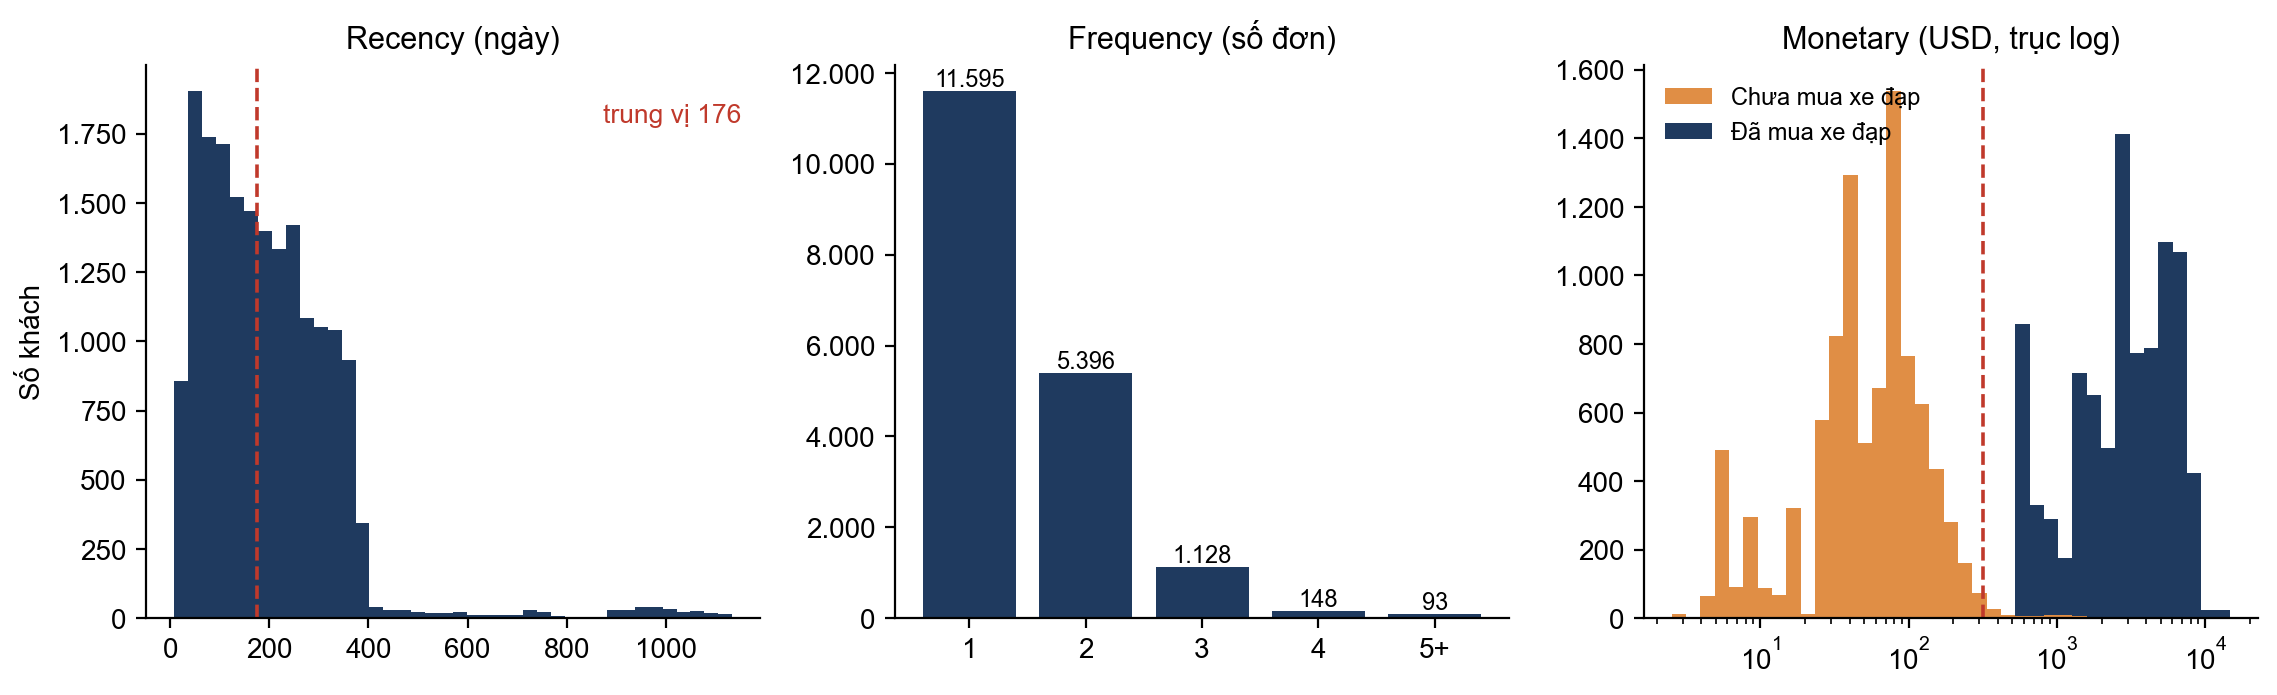
\includegraphics[width=0.85\textwidth]{eda_phan_bo_rfm.png}
\caption{Phân bố Recency, Frequency và Monetary}
\label{fig:phanbo}
\end{figure}

\subsubsection{Quan hệ giữa các thuộc tính}
Hình~\ref{fig:tuongquan} cho hệ số tương quan hạng (Spearman) giữa sáu thuộc tính số: càng gần 1 thì hai thuộc tính càng cùng tăng giảm, càng gần 0 thì càng không liên quan.
\begin{itemize}
    \item Monetary và AOV gần như đi cùng nhau (0,96), nên AOV không cho thêm thông tin.
    \item Recency gần như không liên quan đến Monetary (0,03) và Frequency ($-0{,}18$), nên R, F, M mô tả ba khía cạnh khác nhau.
    \item Các cặp từ 0,7 trở lên trong 11 thuộc tính của mô hình đều gần như trùng nghĩa, ví dụ Share\_Bikes với BikeBuyer (0,87).
\end{itemize}

\begin{figure}[!htbp]
\centering
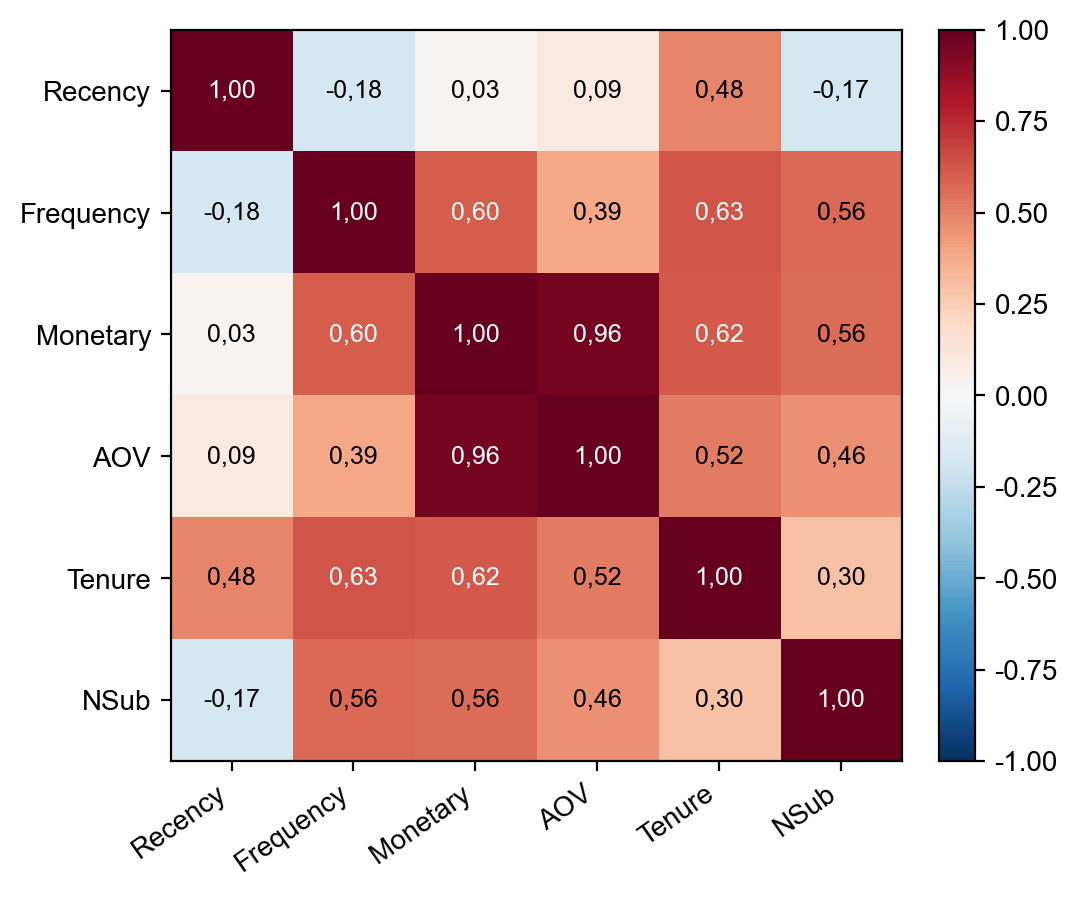
\includegraphics[width=0.55\textwidth]{eda_tuong_quan.png}
\caption{Tương quan hạng Spearman giữa sáu thuộc tính số tại mốc 08/07/2014}
\label{fig:tuongquan}
\end{figure}

\subsubsection{Xu hướng theo thời gian}
Hình~\ref{fig:xuhuongthang} cho thấy số đơn tăng vọt từ tháng 7/2013: khoảng 237 đơn mỗi tháng từ 6/2011 đến 6/2013, rồi khoảng 1.866 đơn mỗi tháng từ 7/2013 đến 5/2014, cao nhất là tháng 5/2014 với 2.209 đơn. Xe đạp chỉ chiếm 15.050 trong 59.795 dòng chi tiết nhưng tạo ra 96,5\% giá trị, còn phụ kiện chiếm nhiều dòng nhất (35.719) nhưng giá trị nhỏ. Tháng 6/2014 bất thường: 930 đơn nhưng không có xe đạp nào, nên doanh thu chỉ khoảng 48,7 nghìn USD. Vì vậy nhóm không dùng tháng 6/2014 để xác định khách rời bỏ.

\begin{figure}[!htbp]
\centering
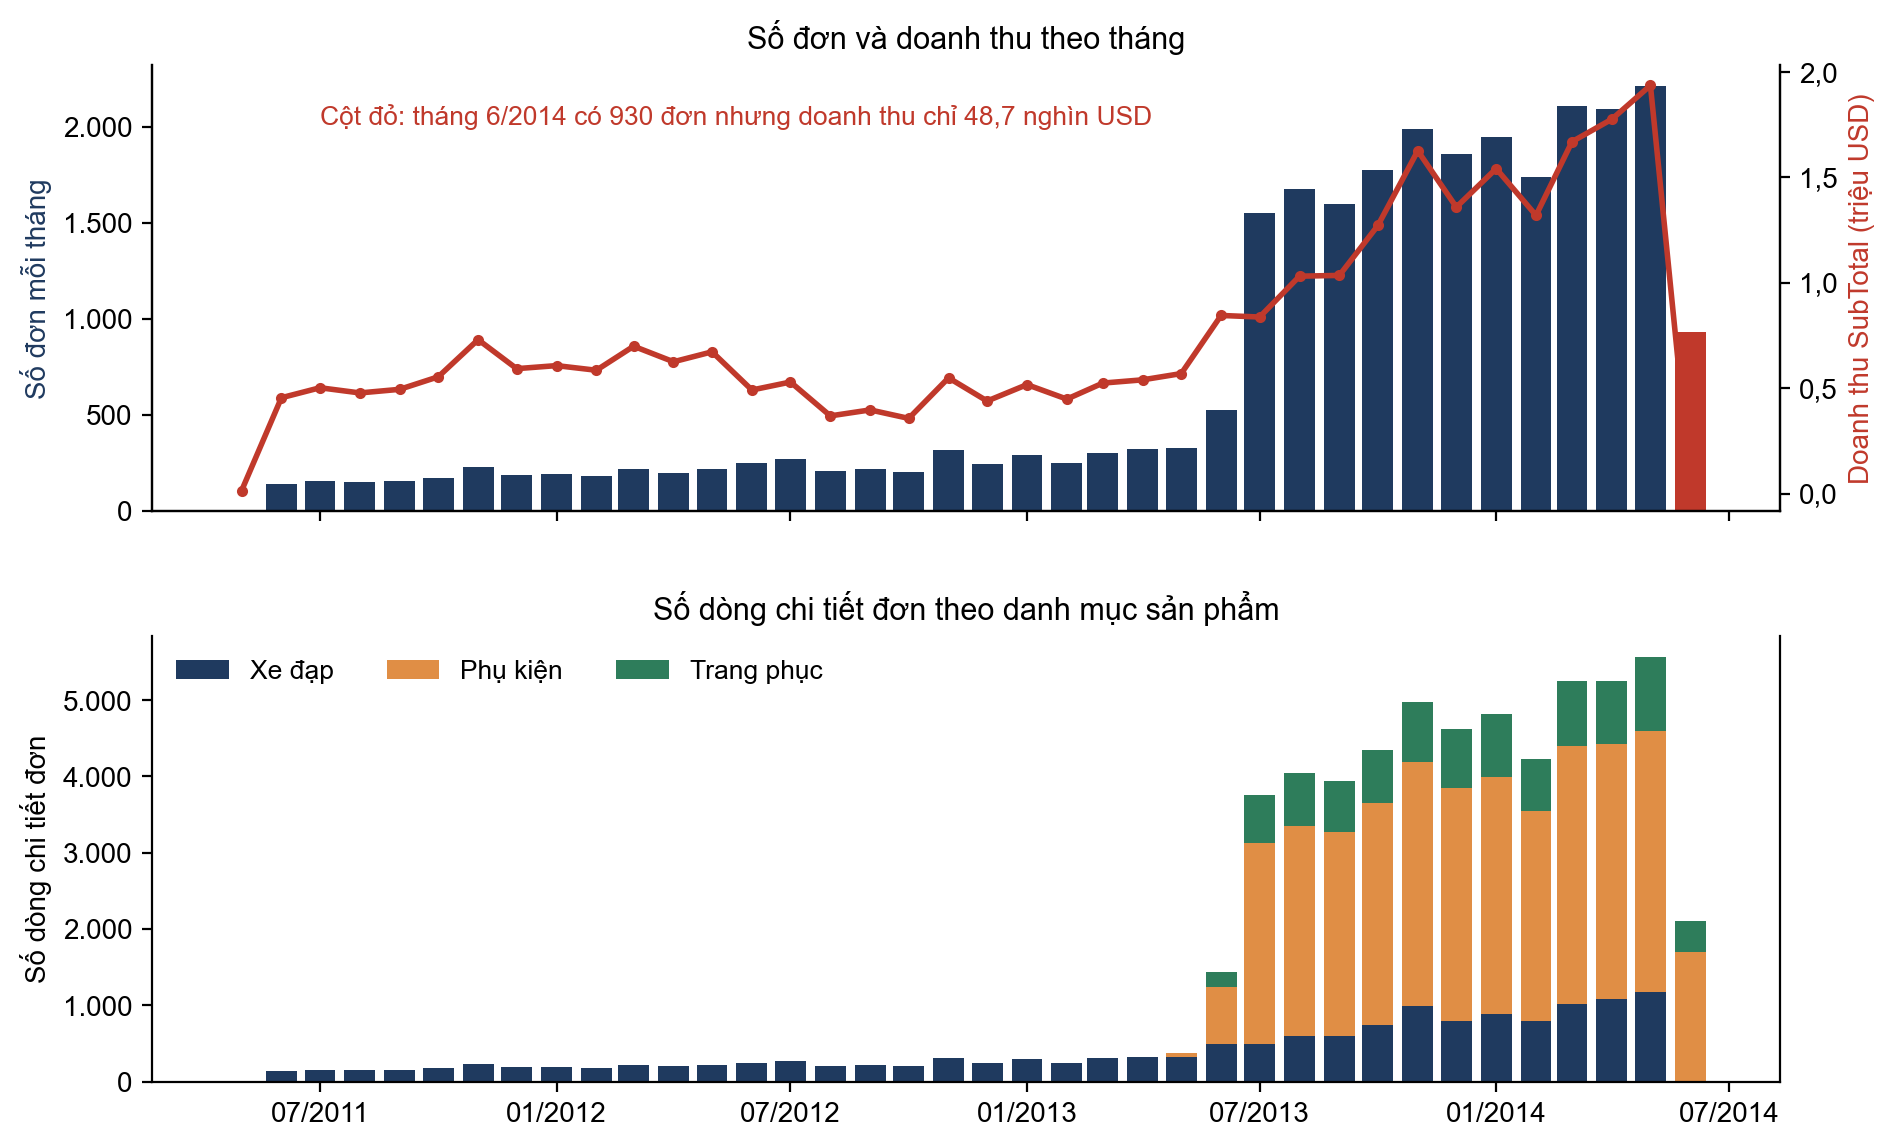
\includegraphics[width=0.75\textwidth]{eda_xu_huong_thang.png}
\caption{Số đơn, doanh thu và số dòng chi tiết theo nhóm sản phẩm của từng tháng}
\label{fig:xuhuongthang}
\end{figure}

\subsubsection{Khách nào mang lại nhiều tiền}
Hình~\ref{fig:pareto} xếp 18.360 khách từ chi tiêu nhiều đến ít. Tiền tập trung vào một số khách nhưng không cực đoan như quy tắc 80/20: 10\% khách đầu mang lại 40,2\% tổng chi tiêu, và cần 28,0\% khách để đạt 80\%. Nhóm chia khách thành ba hạng theo chi tiêu cộng dồn.
\begin{itemize}
    \item \textbf{Hạng A:} 5.137 khách (Monetary từ 2.649,85 USD), tạo ra 80\% tổng chi tiêu.
    \item \textbf{Hạng B:} 2.581 khách (từ 895,40 USD), tạo ra 15\% tiếp theo.
    \item \textbf{Hạng C:} 10.642 khách, chiếm 58,0\% số khách nhưng chỉ mang lại 5\% tổng chi tiêu.
\end{itemize}
Các hạng này dùng ở các chương sau để ưu tiên chăm sóc.

\begin{figure}[!htbp]
\centering
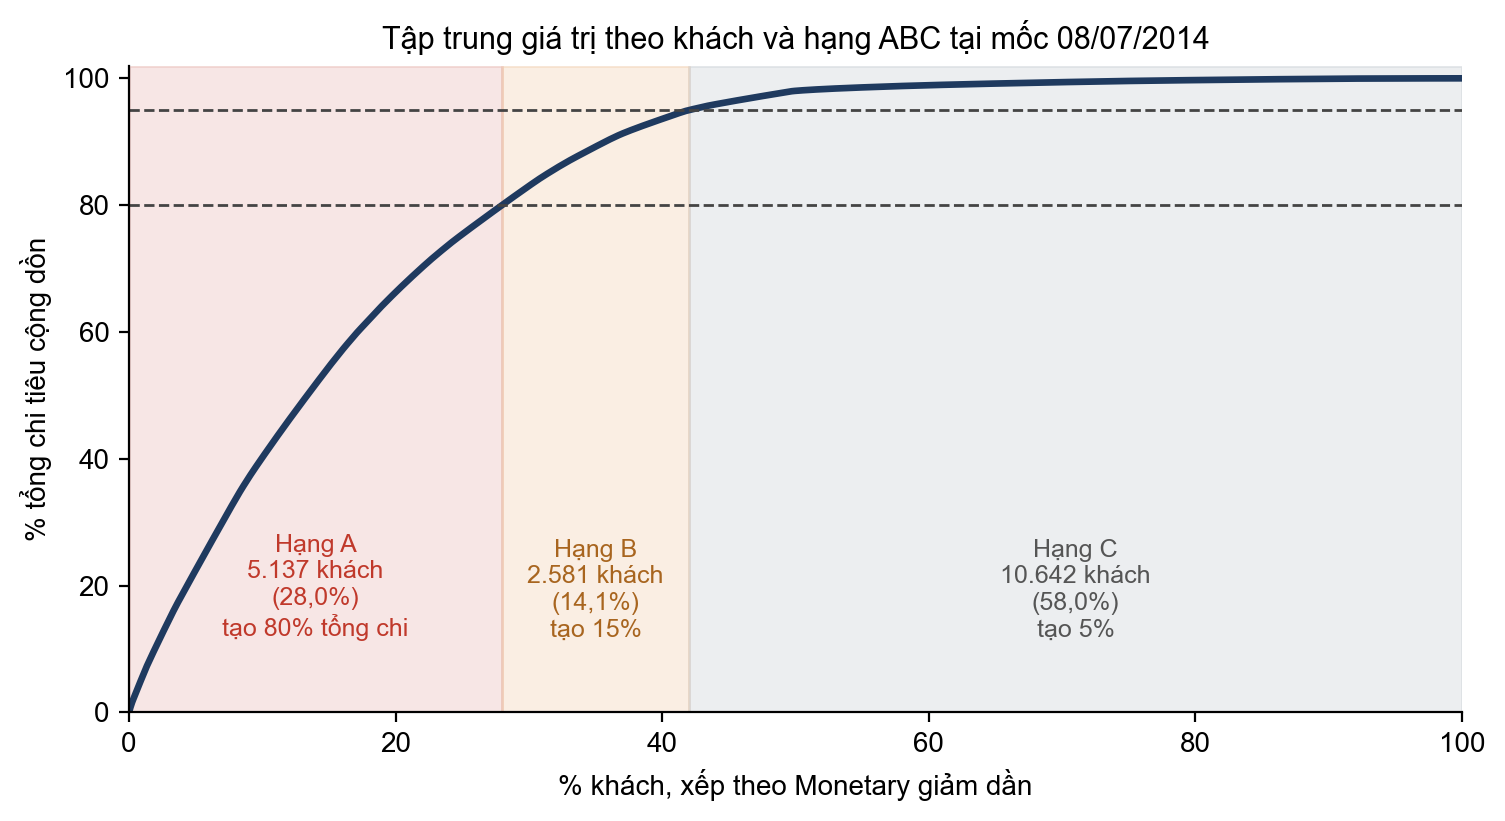
\includegraphics[width=0.65\textwidth]{eda_pareto.png}
\caption{Chi tiêu cộng dồn theo phần trăm khách và ba hạng A, B, C}
\label{fig:pareto}
\end{figure}

\subsection{Xác định khách rời bỏ}
Dữ liệu không có sẵn nhãn rời bỏ nên nhóm tự định nghĩa từ lịch sử mua. Một khách có nhãn $y=1$ (có nguy cơ rời bỏ) nếu sau mốc $T$ khách không đặt đơn nào trong 90 ngày, ngược lại là $y=0$:
\[
y = \begin{cases} 1 & \text{nếu khách không đặt đơn nào trong khoảng } [T,\, T+90) \\ 0 & \text{nếu có đặt ít nhất một đơn.} \end{cases}
\]
Chỉ khách đã có ít nhất một đơn đã gửi trước $T$ mới được gán nhãn. Một mốc $T$ chỉ dùng để huấn luyện mô hình khi đủ hai điều kiện.
\begin{itemize}
    \item \textbf{Đủ thời gian để biết nhãn.} Mốc kiểm tra $E$ phải muộn hơn $T$ ít nhất 97 ngày ($T+97 \leq E$). Lý do là hàng được gửi sau ngày đặt đúng 7 ngày và Snapshot chỉ tính đơn đã gửi, nên đơn đặt ở ngày cuối của 90 ngày ($T+89$) chỉ thấy được từ ngày $T+97$.
    \item \textbf{Không dùng tháng 6/2014.} Cửa sổ 90 ngày phải kết thúc trước 01/06/2014, vì tháng này không có xe đạp.
\end{itemize}
Nhờ vậy 19 mốc từ 01/06/2013 đến 01/03/2014 có nhãn đầy đủ, còn mốc 08/07/2014 chỉ có thuộc tính để dự đoán.

Qua các mốc huấn luyện, số khách tăng từ 5.324 lên 14.167, tỷ lệ $y=1$ luôn quanh 79,3\% đến 82,8\% nhưng cơ cấu khách đổi nhiều: khách chỉ mua một đơn giảm từ 100\% xuống 69,3\%, khách mua từ hai nhóm sản phẩm nhỏ trở lên tăng từ 0\% lên 64,9\%. Vì vậy mô hình được huấn luyện lại ở mỗi kỳ. Tỷ lệ $y=1$ cao cũng nghĩa là một mô hình luôn đoán ``rời bỏ'' đã đúng khoảng 82\%, nên không thể so sánh các mô hình chỉ bằng độ chính xác tổng thể. Nhóm giữ nguyên tỷ lệ này, không lấy mẫu lại hay đổi trọng số hai lớp, vì ở các chương sau xác suất dự đoán được dùng trực tiếp để tính giá trị kinh tế.

\subsection{Chia dữ liệu theo thời gian}
Dữ liệu huấn luyện mô hình và dữ liệu thử mô hình được chia theo thời gian chứ không chia ngẫu nhiên, vì mục tiêu là dự đoán cho tương lai. Mỗi lần thử dùng một cặp mốc $(E \leftarrow T)$, gọi là một fold: mô hình học tại mốc huấn luyện $T$ rồi dự đoán cho khách tại mốc đánh giá $E$ muộn hơn, với $T+97 \leq E$. Bảng~\ref{tab:fold} gồm bốn cặp dùng để phát triển và chọn mô hình, cộng cặp cuối dùng cho lần dự đoán thật ngày 08/07/2014. Hình~\ref{fig:thoigian} vẽ lịch này, thanh màu là cửa sổ 90 ngày và tam giác là mốc đánh giá.

\begin{table}[H]
\centering
\caption{Bốn cặp mốc phát triển và cặp mốc dự đoán thật}
\label{tab:fold}
\footnotesize
\resizebox{\textwidth}{!}{\begin{tabular}{lrrlrrl}
\toprule
Mốc huấn luyện & Số khách & $y=1$ & Mốc đánh giá & Số khách & $y=1$ & Cửa sổ nhãn của mốc huấn luyện \\
\midrule
01/09/2013 & 7.705 & 79,5\% & 15/12/2013 & 11.564 & 81,8\% & 01/09/2013 đến 29/11/2013 \\
01/10/2013 & 8.812 & 79,4\% & 15/01/2014 & 12.617 & 81,8\% & 01/10/2013 đến 29/12/2013 \\
01/11/2013 & 9.898 & 79,4\% & 15/02/2014 & 13.694 & 82,1\% & 01/11/2013 đến 29/01/2014 \\
15/11/2013 & 10.447 & 80,7\% & 01/03/2014 & 14.167 & 82,0\% & 15/11/2013 đến 12/02/2014 \\
01/03/2014 & 14.167 & 82,0\% & 08/07/2014 & 18.360 & -- & 01/03/2014 đến 29/05/2014 \\
\bottomrule
\end{tabular}
}
\end{table}

\begin{figure}[!htbp]
\centering
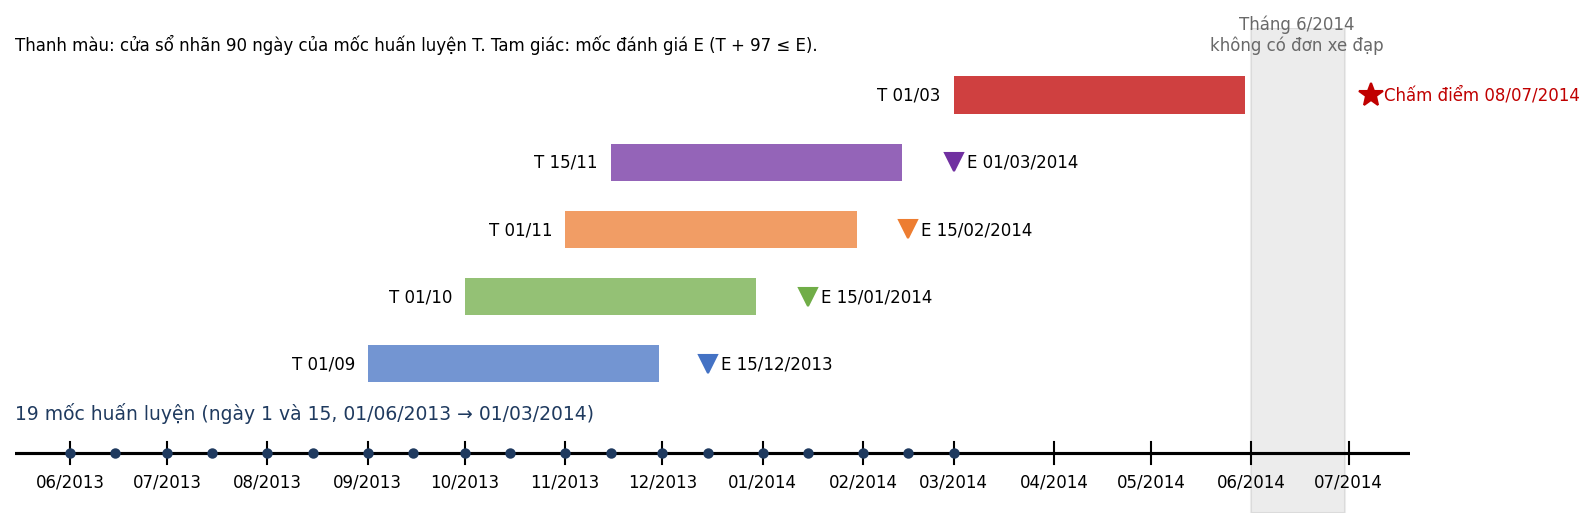
\includegraphics[width=0.8\textwidth]{moc_thoi_gian.png}
\caption{Lịch các mốc huấn luyện, cửa sổ nhãn 90 ngày và mốc đánh giá}
\label{fig:thoigian}
\end{figure}

\subsection{Chia thuộc tính thành khoảng}
Mô hình Naive Bayes làm việc với nhóm giá trị, nên R, F, M được chia thành các khoảng trước khi huấn luyện mô hình. Monetary được chia thành bốn nhóm có số khách xấp xỉ bằng nhau (theo tứ phân vị). Tại mốc huấn luyện 01/03/2014, ba ranh giới là 60,75 USD, 666,86 USD và 3.023,74 USD. Các ranh giới chỉ tính trên mốc huấn luyện rồi giữ nguyên cho mốc đánh giá và mốc dự đoán thật, để mô hình không biết trước tương lai. Với mạng nơ-ron, thuộc tính số được chuẩn hoá z-score (trừ trung bình, chia độ lệch chuẩn) theo cùng nguyên tắc, còn hồi quy logistic dùng cùng các khoảng như Naive Bayes.

Hình~\ref{fig:ytheokhoang} cho thấy quan hệ giữa thuộc tính và nhãn không theo một đường thẳng. Khách mới mua trong 270 ngày gần nhất có tỷ lệ $y=1$ từ 88,9\% đến 91,9\%, còn khách đã từ 270 ngày không mua chỉ có 28,5\% đến 36,7\%. Ở bốn mốc trước đó, tỷ lệ của hai khoảng 270 đến 364 ngày và 365 đến 539 ngày là 46\% đến 72\%. Vậy đây không phải chu kỳ mua dài của khách mà do thành phần khách khác nhau ở từng mốc.

Monetary và BikeBuyer liên quan rất chặt (hệ số Cramér $V$, đo mức liên hệ giữa hai thuộc tính từ 0 đến 1, là 0,923), trong khi Naive Bayes coi các thuộc tính độc lập nên hai thuộc tính này bị tính trùng. Nhóm thử bỏ BikeBuyer (chọn tập con thuộc tính): ROC-AUC tăng từ 0,720 lên 0,729, Brier giảm từ 0,1252 xuống 0,1237 và ECE giảm từ 0,062 xuống 0,048 ở cả bốn cặp mốc (ba chỉ số này định nghĩa ở mục~\ref{sec:chisobosung}), nhưng giá trị ròng $Z$, tiêu chí kinh doanh của đề tài (mục 5.1.2), giảm trung bình 830 USD (khoảng 0,3\%). Vì chênh lệch nhỏ nên nhóm giữ BikeBuyer và ghi nhận đây là một sự đánh đổi (Bảng~\ref{tab:tapthuoctinh}).

\begin{figure}[!htbp]
\centering
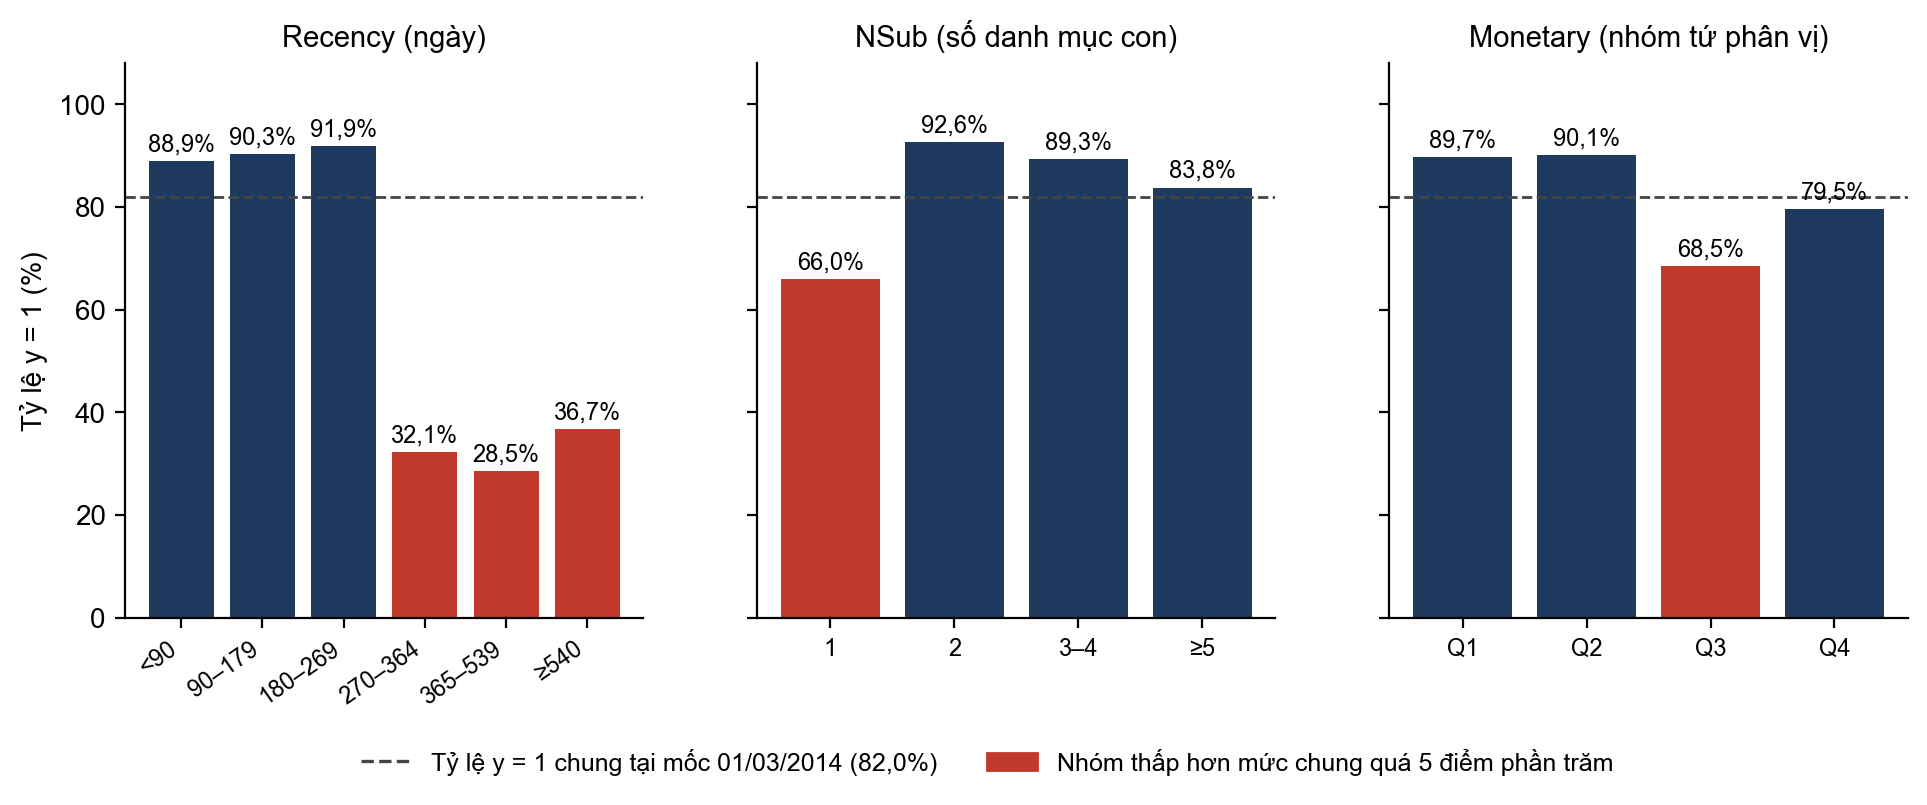
\includegraphics[width=0.7\textwidth]{eda_y_theo_khoang.png}
\caption{Tỷ lệ $y=1$ theo khoảng của Recency, NSub và Monetary}
\label{fig:ytheokhoang}
\end{figure}

\begin{figure}[!tb]
\centering
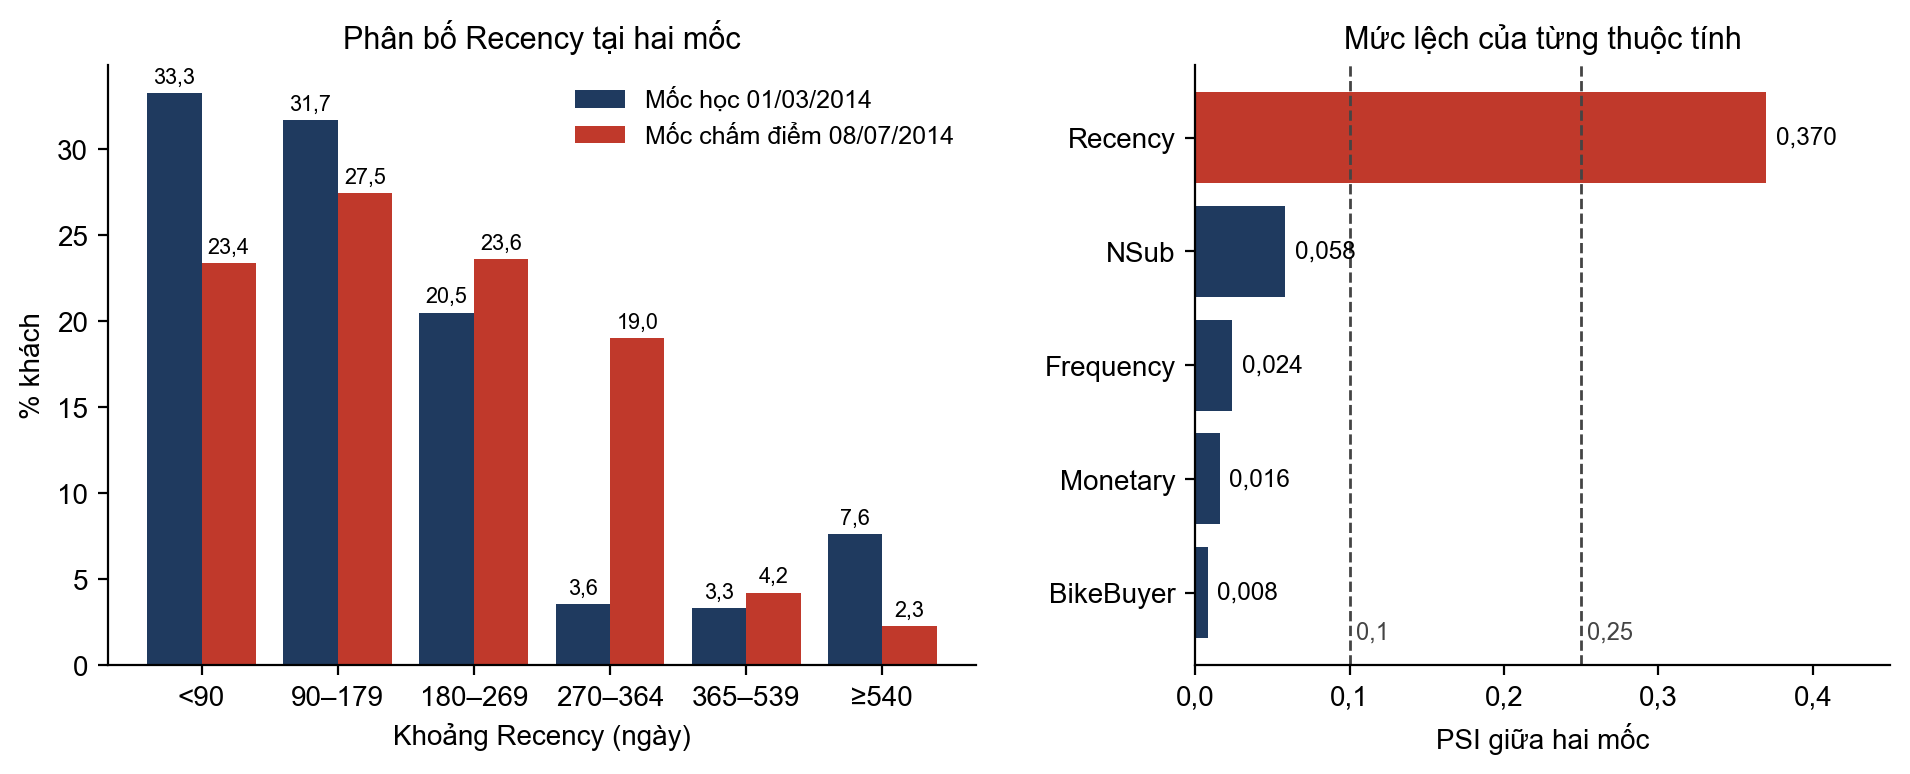
\includegraphics[width=0.42\textwidth]{eda_lech_moc.png}
\caption{Phân bố Recency và PSI của từng thuộc tính giữa mốc huấn luyện và mốc dự đoán}
\label{fig:lechmoc}
\end{figure}

\subsection{Mốc dự đoán có khác mốc huấn luyện không}
Mô hình học tại mốc 01/03/2014 rồi dự đoán tại mốc 08/07/2014, cách nhau 129 ngày, trong khi bốn cặp thử cách nhau 105 đến 106 ngày. Neslin và cộng sự~\cite{neslin2006} ghi nhận trên một cuộc thi dự đoán churn rằng mô hình gần như không giảm độ chính xác khi đem dùng cho dữ liệu thu ba tháng sau tập huấn luyện. Khoảng cách ở đây dài hơn thế, nên nhóm so sánh phân bố giữa hai mốc bằng chỉ số PSI (Population Stability Index, đo mức khác nhau giữa hai phân bố qua các khoảng giá trị, Hình~\ref{fig:lechmoc}), quy ước thường dùng là dưới 0,1 thì hai phân bố giống nhau và trên 0,25 thì khác nhiều.
\begin{itemize}
    \item Recency khác nhiều nhất, PSI là 0,37. Các thuộc tính còn lại đều dưới 0,06.
    \item Khoảng 270 đến 364 ngày chiếm 3,6\% khách ở mốc huấn luyện nhưng 19,0\% ở mốc dự đoán, vì nhóm khách đợt tăng vọt tháng 7/2013 nay rơi vào khoảng này.
    \item Mức khác này không mới: ở bốn cặp thử, PSI của Recency đã là 0,23 đến 0,31.
\end{itemize}
Tuy vậy xác suất của khoảng 270 đến 364 ngày chỉ dựa trên 507 khách của mốc huấn luyện, nên xác suất không mua lại (\texttt{RiskScore}, Chương 5) của nhóm này cần đọc thận trọng.


\textbf{Kiểm tra trước khi huấn luyện.} Nhóm tính lại 10 thuộc tính của 196.985 dòng Snapshot bằng Python, độc lập với SQL, và kết quả khớp hoàn toàn với bảng trong kho. Mười phép kiểm tra miền giá trị đều đạt, ví dụ Tenure không nhỏ hơn Recency và tổng tỷ trọng các nhóm sản phẩm bằng 1.
